% IEEE two-column manuscript (IEEEtran, journal mode), formatted to the IEEE Transactions author instructions.
% Figures for this manuscript are in ./figures (FIG_PROFILE=ieee python scripts/final_report.py; same for round2_tables.py).
% Numbers come from ../numbers.tex (scripts/final_report.py) and ../numbers_r2.tex (scripts/round2_tables.py); do not retype them.
\documentclass[journal]{IEEEtran}
\usepackage{mathptmx}  % Times-compatible math so that numbers inside $...$ match the text font
\usepackage{amsmath,amssymb,booktabs,graphicx,cite,array}
\usepackage{dblfloatfix}  % lets wide figures and tables sit at the bottom of a page
\usepackage[hidelinks]{hyperref}
\graphicspath{{figures/}}
% auto-generated by scripts/final_report.py -- do not edit
\newcommand{\TErmAurocAll}{0.733}
\newcommand{\TErmAurocDev}{0.758}
\newcommand{\TErmAurocConf}{0.707}
\newcommand{\TErmWorstFold}{0.565}
\newcommand{\TErmBalAcc}{0.634}
\newcommand{\TErmEce}{0.157}
\newcommand{\TErmDiffVsErm}{0.000}
\newcommand{\TGroupdroAurocAll}{0.748}
\newcommand{\TGroupdroAurocDev}{0.761}
\newcommand{\TGroupdroAurocConf}{0.735}
\newcommand{\TGroupdroWorstFold}{0.657}
\newcommand{\TGroupdroBalAcc}{0.689}
\newcommand{\TGroupdroEce}{0.144}
\newcommand{\TGroupdroDiffVsErm}{0.015}
\newcommand{\TGroupdroLo}{\ensuremath{-}0.015}
\newcommand{\TGroupdroHi}{0.055}
\newcommand{\TGroupdroFoldsBetter}{4}
\newcommand{\TDannAurocAll}{0.727}
\newcommand{\TDannAurocDev}{0.752}
\newcommand{\TDannAurocConf}{0.702}
\newcommand{\TDannWorstFold}{0.645}
\newcommand{\TDannBalAcc}{0.599}
\newcommand{\TDannEce}{0.166}
\newcommand{\TDannDiffVsErm}{\ensuremath{-}0.006}
\newcommand{\TDannLo}{\ensuremath{-}0.049}
\newcommand{\TDannHi}{0.035}
\newcommand{\TDannFoldsBetter}{4}
\newcommand{\TGenericAugAurocAll}{0.732}
\newcommand{\TGenericAugAurocDev}{0.748}
\newcommand{\TGenericAugAurocConf}{0.716}
\newcommand{\TGenericAugWorstFold}{0.619}
\newcommand{\TGenericAugBalAcc}{0.663}
\newcommand{\TGenericAugEce}{0.150}
\newcommand{\TGenericAugDiffVsErm}{\ensuremath{-}0.001}
\newcommand{\TGenericAugLo}{\ensuremath{-}0.029}
\newcommand{\TGenericAugHi}{0.032}
\newcommand{\TGenericAugFoldsBetter}{3}
\newcommand{\TSiteProfileAugAurocAll}{0.726}
\newcommand{\TSiteProfileAugAurocDev}{0.757}
\newcommand{\TSiteProfileAugAurocConf}{0.694}
\newcommand{\TSiteProfileAugWorstFold}{0.641}
\newcommand{\TSiteProfileAugBalAcc}{0.618}
\newcommand{\TSiteProfileAugEce}{0.174}
\newcommand{\TSiteProfileAugDiffVsErm}{\ensuremath{-}0.007}
\newcommand{\TSiteProfileAugLo}{\ensuremath{-}0.060}
\newcommand{\TSiteProfileAugHi}{0.038}
\newcommand{\TSiteProfileAugFoldsBetter}{6}
\newcommand{\TProfileAdversaryPaiAurocAll}{0.730}
\newcommand{\TProfileAdversaryPaiAurocDev}{0.753}
\newcommand{\TProfileAdversaryPaiAurocConf}{0.708}
\newcommand{\TProfileAdversaryPaiWorstFold}{0.551}
\newcommand{\TProfileAdversaryPaiBalAcc}{0.615}
\newcommand{\TProfileAdversaryPaiEce}{0.154}
\newcommand{\TProfileAdversaryPaiDiffVsErm}{\ensuremath{-}0.002}
\newcommand{\TProfileAdversaryPaiLo}{\ensuremath{-}0.020}
\newcommand{\TProfileAdversaryPaiHi}{0.014}
\newcommand{\TProfileAdversaryPaiFoldsBetter}{4}
\newcommand{\TSidlCcAurocAll}{0.711}
\newcommand{\TSidlCcAurocDev}{0.722}
\newcommand{\TSidlCcAurocConf}{0.699}
\newcommand{\TSidlCcWorstFold}{0.635}
\newcommand{\TSidlCcBalAcc}{0.612}
\newcommand{\TSidlCcEce}{0.178}
\newcommand{\TSidlCcDiffVsErm}{\ensuremath{-}0.022}
\newcommand{\TSidlCcLo}{\ensuremath{-}0.069}
\newcommand{\TSidlCcHi}{0.030}
\newcommand{\TSidlCcFoldsBetter}{3}
\newcommand{\TSidlPhysAurocAll}{0.744}
\newcommand{\TSidlPhysAurocDev}{0.756}
\newcommand{\TSidlPhysAurocConf}{0.732}
\newcommand{\TSidlPhysWorstFold}{0.650}
\newcommand{\TSidlPhysBalAcc}{0.656}
\newcommand{\TSidlPhysEce}{0.192}
\newcommand{\TSidlPhysDiffVsErm}{0.011}
\newcommand{\TSidlPhysLo}{\ensuremath{-}0.016}
\newcommand{\TSidlPhysHi}{0.050}
\newcommand{\TSidlPhysFoldsBetter}{3}
\newcommand{\TSidlFullAurocAll}{0.701}
\newcommand{\TSidlFullAurocDev}{0.738}
\newcommand{\TSidlFullAurocConf}{0.665}
\newcommand{\TSidlFullWorstFold}{0.415}
\newcommand{\TSidlFullBalAcc}{0.590}
\newcommand{\TSidlFullEce}{0.175}
\newcommand{\TSidlFullDiffVsErm}{\ensuremath{-}0.031}
\newcommand{\TSidlFullLo}{\ensuremath{-}0.085}
\newcommand{\TSidlFullHi}{0.016}
\newcommand{\TSidlFullFoldsBetter}{3}
\newcommand{\CLsoCvplusCovMean}{0.942}
\newcommand{\CLsoCvplusCovMin}{0.867}
\newcommand{\CLsoCvplusSize}{1.747}
\newcommand{\CLsoCvplusNUnder}{0}
\newcommand{\CLsoCvplusN}{8}
\newcommand{\CLsoCvplusCovCalibErr}{0.041}
\newcommand{\CLsoCvplusFracUnder}{0.069}
\newcommand{\CLsoCvplusSizeAtCov}{1.602}
\newcommand{\CLsoCvplusBalCovMean}{0.926}
\newcommand{\CLsoCvplusBalCovMin}{0.792}
\newcommand{\CLsoCvplusBalSize}{1.687}
\newcommand{\CLsoCvplusBalNUnder}{1}
\newcommand{\CLsoCvplusBalN}{8}
\newcommand{\CLsoCvplusBalCovCalibErr}{0.020}
\newcommand{\CLsoCvplusBalFracUnder}{0.153}
\newcommand{\CLsoCvplusBalSizeAtCov}{1.603}
\newcommand{\CLsoSplitCovMean}{0.905}
\newcommand{\CLsoSplitCovMin}{0.732}
\newcommand{\CLsoSplitSize}{1.590}
\newcommand{\CLsoSplitNUnder}{1}
\newcommand{\CLsoSplitN}{8}
\newcommand{\CLsoSplitCovCalibErr}{0.011}
\newcommand{\CLsoSplitFracUnder}{0.208}
\newcommand{\CLsoSplitSizeAtCov}{1.574}
\newcommand{\CLsoSplitBalCovMean}{0.886}
\newcommand{\CLsoSplitBalCovMin}{0.711}
\newcommand{\CLsoSplitBalSize}{1.540}
\newcommand{\CLsoSplitBalNUnder}{1}
\newcommand{\CLsoSplitBalN}{8}
\newcommand{\CLsoSplitBalCovCalibErr}{0.009}
\newcommand{\CLsoSplitBalFracUnder}{0.236}
\newcommand{\CLsoSplitBalSizeAtCov}{1.578}
\newcommand{\CLsoWorstCovMean}{0.960}
\newcommand{\CLsoWorstCovMin}{0.832}
\newcommand{\CLsoWorstSize}{1.807}
\newcommand{\CLsoWorstNUnder}{1}
\newcommand{\CLsoWorstN}{8}
\newcommand{\CLsoWorstCovCalibErr}{0.083}
\newcommand{\CLsoWorstFracUnder}{0.028}
\newcommand{\CLsoWorstSizeAtCov}{1.588}
\newcommand{\CPooledCovMean}{0.836}
\newcommand{\CPooledCovMin}{0.743}
\newcommand{\CPooledSize}{1.389}
\newcommand{\CPooledNUnder}{4}
\newcommand{\CPooledN}{8}
\newcommand{\CPooledCovCalibErr}{0.048}
\newcommand{\CPooledFracUnder}{0.389}
\newcommand{\CPooledSizeAtCov}{1.582}
\newcommand{\CSiteBalancedCovMean}{0.840}
\newcommand{\CSiteBalancedCovMin}{0.746}
\newcommand{\CSiteBalancedSize}{1.376}
\newcommand{\CSiteBalancedNUnder}{4}
\newcommand{\CSiteBalancedN}{8}
\newcommand{\CSiteBalancedCovCalibErr}{0.053}
\newcommand{\CSiteBalancedFracUnder}{0.472}
\newcommand{\CSiteBalancedSizeAtCov}{1.603}
\newcommand{\CWorstSiteCovMean}{0.904}
\newcommand{\CWorstSiteCovMin}{0.751}
\newcommand{\CWorstSiteSize}{1.597}
\newcommand{\CWorstSiteNUnder}{2}
\newcommand{\CWorstSiteN}{8}
\newcommand{\CWorstSiteCovCalibErr}{0.009}
\newcommand{\CWorstSiteFracUnder}{0.236}
\newcommand{\CWorstSiteSizeAtCov}{1.582}
\newcommand{\OMeanSignedSeen}{0.118}
\newcommand{\OMeanSignedLso}{0.007}
\newcommand{\OMaeSeen}{0.130}
\newcommand{\OMaeLso}{0.070}
\newcommand{\ONUnits}{16}
\newcommand{\ORhoSeen}{\ensuremath{-}0.310}
\newcommand{\ORhoLso}{\ensuremath{-}0.048}
\newcommand{\ORhoGapCov}{\ensuremath{-}0.452}
\newcommand{\datasetTotal}{924}
\newcommand{\profLeakLogreg}{0.662}
\newcommand{\profLeakGbm}{0.588}
\newcommand{\priorSpreadSd}{0.274}
\newcommand{\siteAccProfile}{0.367}
\newcommand{\siteAccChance}{0.224}
\newcommand{\synthDiffErmP}{\ensuremath{-}0.000}
\newcommand{\synthDiffErmPLo}{\ensuremath{-}0.040}
\newcommand{\synthDiffErmPHi}{0.038}
\newcommand{\synthDiffDann}{\ensuremath{-}0.092}
\newcommand{\synthDiffDannLo}{\ensuremath{-}0.175}
\newcommand{\synthDiffDannHi}{\ensuremath{-}0.016}
\newcommand{\synthDiffCdann}{\ensuremath{-}0.077}
\newcommand{\synthDiffCdannLo}{\ensuremath{-}0.142}
\newcommand{\synthDiffCdannHi}{\ensuremath{-}0.019}
\newcommand{\synthDiffCdannP}{\ensuremath{-}0.047}
\newcommand{\synthDiffCdannPLo}{\ensuremath{-}0.092}
\newcommand{\synthDiffCdannPHi}{\ensuremath{-}0.013}
\newcommand{\rankCorrDevConf}{0.500}
\newcommand{\relErm}{0.438}
\newcommand{\relGroupdro}{0.423}
\newcommand{\relDann}{0.415}
\newcommand{\relGenericAug}{0.411}
\newcommand{\relSiteProfileAug}{0.396}
\newcommand{\relProfileAdversaryPai}{0.398}
\newcommand{\relSidlCc}{0.473}
\newcommand{\relSidlPhys}{0.422}
\newcommand{\relSidlFull}{0.514}
\newcommand{\ensAurocFull}{0.733}
\newcommand{\ensAurocEns}{0.748}
\newcommand{\ensDAuroc}{0.016}
\newcommand{\ensDAurocLo}{\ensuremath{-}0.008}
\newcommand{\ensDAurocHi}{0.049}
\newcommand{\ensDEce}{\ensuremath{-}0.003}
\newcommand{\ensFoldsBetter}{5}
\newcommand{\ensMembers}{9}

% auto-generated by scripts/round2_tables.py -- do not edit
\newcommand{\RtCnnDev}{0.755}
\newcommand{\RtCnnConf}{0.699}
\newcommand{\RtCnnAll}{0.727}
\newcommand{\RtCnnWorst}{0.595}
\newcommand{\RtPreDev}{0.739}
\newcommand{\RtPreConf}{0.758}
\newcommand{\RtPreAll}{0.749}
\newcommand{\RtPreWorst}{0.619}
\newcommand{\RtCnnEnsDev}{0.772}
\newcommand{\RtCnnEnsConf}{0.716}
\newcommand{\RtCnnEnsAll}{0.744}
\newcommand{\RtCnnEnsWorst}{0.617}
\newcommand{\RtPreEnsDev}{0.750}
\newcommand{\RtPreEnsConf}{0.771}
\newcommand{\RtPreEnsAll}{0.760}
\newcommand{\RtPreEnsWorst}{0.646}
\newcommand{\RtEnsDev}{0.789}
\newcommand{\RtEnsConf}{0.770}
\newcommand{\RtEnsAll}{0.780}
\newcommand{\RtEnsWorst}{0.671}
\newcommand{\RtEnsVsCnnEnsDev}{+0.017}
\newcommand{\RtEnsVsCnnEnsDevLo}{\ensuremath{-}0.050}
\newcommand{\RtEnsVsCnnEnsDevHi}{+0.096}
\newcommand{\RtEnsVsCnnEnsConf}{+0.055}
\newcommand{\RtEnsVsCnnEnsConfLo}{\ensuremath{-}0.062}
\newcommand{\RtEnsVsCnnEnsConfHi}{+0.181}
\newcommand{\RtEnsVsCnnEnsAll}{+0.036}
\newcommand{\RtEnsVsCnnEnsAllLo}{\ensuremath{-}0.031}
\newcommand{\RtEnsVsCnnEnsAllHi}{+0.110}
\newcommand{\RtEnsVsCnnDev}{+0.034}
\newcommand{\RtEnsVsCnnDevLo}{\ensuremath{-}0.034}
\newcommand{\RtEnsVsCnnDevHi}{+0.111}
\newcommand{\RtEnsVsCnnConf}{+0.071}
\newcommand{\RtEnsVsCnnConfLo}{\ensuremath{-}0.043}
\newcommand{\RtEnsVsCnnConfHi}{+0.194}
\newcommand{\RtEnsVsCnnAll}{+0.053}
\newcommand{\RtEnsVsCnnAllLo}{\ensuremath{-}0.013}
\newcommand{\RtEnsVsCnnAllHi}{+0.129}
\newcommand{\RtPreVsCnnDev}{\ensuremath{-}0.015}
\newcommand{\RtPreVsCnnDevLo}{\ensuremath{-}0.122}
\newcommand{\RtPreVsCnnDevHi}{+0.105}
\newcommand{\RtPreVsCnnConf}{+0.059}
\newcommand{\RtPreVsCnnConfLo}{\ensuremath{-}0.114}
\newcommand{\RtPreVsCnnConfHi}{+0.245}
\newcommand{\RtPreVsCnnAll}{+0.022}
\newcommand{\RtPreVsCnnAllLo}{\ensuremath{-}0.079}
\newcommand{\RtPreVsCnnAllHi}{+0.133}
\newcommand{\RtEnsVsPreEnsDev}{+0.039}
\newcommand{\RtEnsVsPreEnsDevLo}{\ensuremath{-}0.005}
\newcommand{\RtEnsVsPreEnsDevHi}{+0.080}
\newcommand{\RtEnsVsPreEnsConf}{\ensuremath{-}0.001}
\newcommand{\RtEnsVsPreEnsConfLo}{\ensuremath{-}0.069}
\newcommand{\RtEnsVsPreEnsConfHi}{+0.066}
\newcommand{\RtEnsVsPreEnsAll}{+0.019}
\newcommand{\RtEnsVsPreEnsAllLo}{\ensuremath{-}0.023}
\newcommand{\RtEnsVsPreEnsAllHi}{+0.058}
\newcommand{\RtCnnEnsVsCnnDev}{+0.017}
\newcommand{\RtCnnEnsVsCnnDevLo}{+0.002}
\newcommand{\RtCnnEnsVsCnnDevHi}{+0.032}
\newcommand{\RtCnnEnsVsCnnConf}{+0.016}
\newcommand{\RtCnnEnsVsCnnConfLo}{+0.000}
\newcommand{\RtCnnEnsVsCnnConfHi}{+0.034}
\newcommand{\RtCnnEnsVsCnnAll}{+0.017}
\newcommand{\RtCnnEnsVsCnnAllLo}{+0.006}
\newcommand{\RtCnnEnsVsCnnAllHi}{+0.030}
\newcommand{\RtGdroDiff}{+0.018}
\newcommand{\RtGdroLo}{\ensuremath{-}0.000}
\newcommand{\RtGdroHi}{+0.039}
\newcommand{\RtCenterDiff}{\ensuremath{-}0.040}
\newcommand{\RtCenterLo}{\ensuremath{-}0.076}
\newcommand{\RtCenterHi}{\ensuremath{-}0.006}
\newcommand{\RtCdannPDiff}{\ensuremath{-}0.025}
\newcommand{\RtCdannPLo}{\ensuremath{-}0.062}
\newcommand{\RtCdannPHi}{+0.005}
\newcommand{\RtCcFullDiff}{\ensuremath{-}0.006}
\newcommand{\RtCcFullLo}{\ensuremath{-}0.026}
\newcommand{\RtCcFullHi}{+0.011}
\newcommand{\RtGdroDev}{+0.021}
\newcommand{\RtGdroConf}{+0.016}
\newcommand{\RtFeatErmDev}{0.739}
\newcommand{\RcCnnPooledCov}{0.836}
\newcommand{\RcCnnPooledUnder}{4}
\newcommand{\RcCnnPooledSize}{1.39}
\newcommand{\RcCnnPooledMin}{0.743}
\newcommand{\RcCnnPooledSninety}{1.58}
\newcommand{\RcCnnCvplusCov}{0.942}
\newcommand{\RcCnnCvplusUnder}{0}
\newcommand{\RcCnnCvplusSize}{1.75}
\newcommand{\RcCnnCvplusMin}{0.867}
\newcommand{\RcCnnCvplusSninety}{1.60}
\newcommand{\RcCnnWorstCov}{0.904}
\newcommand{\RcCnnWorstUnder}{2}
\newcommand{\RcCnnWorstSize}{1.60}
\newcommand{\RcCnnWorstMin}{0.751}
\newcommand{\RcCnnWorstSninety}{1.58}
\newcommand{\RcPrePooledCov}{0.834}
\newcommand{\RcPrePooledUnder}{5}
\newcommand{\RcPrePooledSize}{1.32}
\newcommand{\RcPrePooledMin}{0.766}
\newcommand{\RcPrePooledSninety}{1.55}
\newcommand{\RcPreCvplusCov}{0.937}
\newcommand{\RcPreCvplusUnder}{0}
\newcommand{\RcPreCvplusSize}{1.68}
\newcommand{\RcPreCvplusMin}{0.862}
\newcommand{\RcPreCvplusSninety}{1.51}
\newcommand{\RcPreWorstCov}{0.890}
\newcommand{\RcPreWorstUnder}{1}
\newcommand{\RcPreWorstSize}{1.52}
\newcommand{\RcPreWorstMin}{0.795}
\newcommand{\RcPreWorstSninety}{1.57}
\newcommand{\RcEnsPooledCov}{0.836}
\newcommand{\RcEnsPooledUnder}{5}
\newcommand{\RcEnsPooledSize}{1.29}
\newcommand{\RcEnsPooledMin}{0.773}
\newcommand{\RcEnsPooledSninety}{1.48}
\newcommand{\RcEnsCvplusCov}{0.936}
\newcommand{\RcEnsCvplusUnder}{0}
\newcommand{\RcEnsCvplusSize}{1.63}
\newcommand{\RcEnsCvplusMin}{0.870}
\newcommand{\RcEnsCvplusSninety}{1.52}
\newcommand{\RcEnsWorstCov}{0.889}
\newcommand{\RcEnsWorstUnder}{2}
\newcommand{\RcEnsWorstSize}{1.48}
\newcommand{\RcEnsWorstMin}{0.773}
\newcommand{\RcEnsWorstSninety}{1.52}
\newcommand{\RcEnsCnnCvplusDiff}{\ensuremath{-}0.059}
\newcommand{\RcEnsCnnCvplusLo}{\ensuremath{-}0.120}
\newcommand{\RcEnsCnnCvplusHi}{+0.002}
\newcommand{\RcEnsCnnCvplusN}{6}
\newcommand{\RcEnsCnnPooledDiff}{\ensuremath{-}0.042}
\newcommand{\RcEnsCnnPooledLo}{\ensuremath{-}0.123}
\newcommand{\RcEnsCnnPooledHi}{+0.042}
\newcommand{\RcEnsCnnPooledN}{5}
\newcommand{\RdSiteAcc}{0.473}
\newcommand{\RdSiteMaj}{0.224}
\newcommand{\RdOptim}{0.115}
\newcommand{\RdOptimMae}{0.145}
\newcommand{\RdValAuc}{0.863}
\newcommand{\RdTestAuc}{0.749}

\newcommand{\erm}{ERM}
\newcommand{\tabnote}[1]{\par\vspace{3pt}{\footnotesize\raggedright #1\par}}
\newcommand{\tabin}[1]{\input{../tables/#1}}
\setlength{\tabcolsep}{3pt}
\renewcommand{\arraystretch}{1.05}
\hyphenation{Pre-trained}

\begin{document}
\bstctlcite{IEEEexample:BSTcontrol}

\title{Scanner-Invariant and Institution-Invariant Deep Learning for Reliable Medical Image Diagnosis Across Heterogeneous Clinical Environments}

% TODO(authors): corresponding author, funding statement (IEEE: "This work was supported by ..."), e-mail address, ORCIDs.
\author{K.~Venkateswara~Rao, Ch.~Venkata~Naveen, J.~Harish, and G.~Siva~Rama~Krishna%
\thanks{Manuscript received XX XX, 2026; revised XX XX, 2026; accepted XX XX, 2026. (Corresponding author: XX XX.)}%
\thanks{The authors are with the Department of Computer Science and Engineering, Vignan's Lara Institute of Technology \& Science, Vadlamudi, Guntur District, Andhra Pradesh, India (e-mail: XX).}}

\markboth{Preprint submitted to an IEEE journal}{Rao \MakeLowercase{\textit{et al.}}: Scanner-Invariant and Institution-Invariant Deep Learning for Medical Image Diagnosis}

\maketitle

\begin{abstract}
Diagnostic image models often lose accuracy at hospitals that were absent from their training data. We asked whether making a model invariant to scanner and institution helps at such hospitals, and whether conformal prediction sets stay valid there. We tested both on an open chest-radiograph benchmark (924 images, ten sources, COVID-19 versus other findings), holding out one site at a time. Four sites guided every design decision; the other four were run once with frozen settings. Across eight held-out sites, none of eight training methods beat empirical risk minimization by more than noise, including three variants of our own recipe. The largest gain, from group distributionally robust optimization, was $+\TGroupdroDiffVsErm$ in the area under the receiver operating characteristic curve, with an interval that included zero, and the result repeated on a frozen pretrained encoder. The more useful findings concern evaluation. Five image statistics with no anatomy predicted the diagnosis at unseen sites (area $\profLeakLogreg$). Validation on seen sites overstated the held-out area by $\OMeanSignedSeen$, and standard conformal sets covered only $\CPooledCovMean$ of cases at a $0.90$ target, mainly by missing cases without COVID-19. Calibrating with sites as cross-validation folds removed the worst shortfalls, with sets about $26\%$ larger. Averaging a convolutional network with the pretrained model gave the best mean area ($\RtEnsAll$), but most of that lead came from the two smallest test sites, and no difference survived correction for multiple comparisons. The data are small, cover one modality, and support no claim about clinical COVID-19 detection.
\end{abstract}

\begin{IEEEkeywords}
Conformal prediction, dataset shift, domain generalization, medical diagnostic imaging.
\end{IEEEkeywords}

\section{Introduction}
\IEEEPARstart{A}{ diagnostic} model trained on pooled data from several hospitals can learn cues that identify the hospital instead of the disease~\cite{zech2018variable,degrave2021ai,geirhos2020shortcut}. Such a model looks good on validation images from hospitals it has already seen and then fails quietly at a new one. A common remedy is to make the model invariant to scanner and institution, through adversarial alignment, matching of feature statistics, harmonization, or augmentation~\cite{ganin2016domain,sun2016deep,zhang2020generalizing,johnson2007adjusting}. Whether these remedies work on small, messy, multi-site data is still unclear. Controlled comparisons on hospital chest radiographs and on general benchmarks found that such methods often do not beat plain training~\cite{zhang2021empirical,gulrajani2021in}. We found fewer comparisons on the small, mixed public COVID-19 collections that many studies still use, and none that put the second question below to the same data. That question follows from the first: when a model does fail at a new site, can its uncertainty estimates warn us?

We study four research questions.
\begin{itemize}\setlength\itemsep{0pt}
  \item \textbf{RQ1.} Do invariance methods improve the area under the receiver operating characteristic curve (AUROC) at hospitals unseen in training, when all settings are frozen before the final test?
  \item \textbf{RQ2.} Does the answer change if the encoder is a frozen, pretrained chest-radiograph network instead of a small convolutional neural network (CNN) trained from scratch?
  \item \textbf{RQ3.} Do conformal prediction sets keep their nominal coverage at an unseen site, and does calibrating with sites as the unit help?
  \item \textbf{RQ4.} Why do performance and coverage estimates made on seen sites mislead at a new site?
\end{itemize}

The project began as an attempt to build an invariance recipe, which we call SIDL (scanner- and institution-invariant deep learning). It has three parts. The first is a site adversary that works within each class, so that different disease prevalence across hospitals is not penalized~\cite{zhao2019learning}. The second is augmentation that re-renders an image as if it came from another \emph{observed} site, using statistics estimated from the training images without labels. The third is conformal prediction sets calibrated with an unseen site in mind. We evaluated the recipe with leave-one-site-out (LOSO) testing, a development/confirmation split of the sites, and configurations frozen before the confirmation run.

The recipe did not beat empirical risk minimization (ERM), and neither did the baseline methods. Because a small network trained from scratch is an easy target for that objection, we repeated the study on top of a frozen pretrained chest-radiograph encoder, and the answer stayed the same. We report this frozen negative result because it is useful to anyone choosing among these methods on small multi-site data, and we pair it with the evaluation findings that explain what went wrong and how to report uncertainty at unseen sites. Our contributions are modest, and we mark novelty carefully because our literature search was targeted and not systematic:
\begin{itemize}\setlength\itemsep{0pt}
  \item a frozen LOSO protocol on open data with a hierarchical paired bootstrap; a negative result for eight methods against \erm{}, repeated on a pretrained encoder family; and a controlled label-shift sweep;
  \item two label-free diagnostics of acquisition shortcuts, one measuring how much the label leaks into image statistics and one measuring how much a model relies on them;
  \item evidence on calibrating prediction sets for unseen sites, replicated on two encoder families and their ensemble: seen-site validation is optimistic, standard conformal sets under-cover (mostly on non-COVID images), a site-fold cross-validation+ (CV+) rule avoids the worst cases, and simulated shifts do not reproduce the real effect;
  \item a pre-specified comparison showing that averaging a from-scratch CNN with a pretrained model gives a suggestive but not significant gain, which a sensitivity analysis traces mostly to two tiny test sets.
\end{itemize}
We do not claim clinical COVID-19 detection performance. The benchmark is a shortcut-prone stress test.

Section~\ref{sec:related} places the work in the literature, Sections~\ref{sec:methods} and~\ref{sec:protocol} describe the methods, the benchmark, and the protocol, and Section~\ref{sec:results} gives the results. RQ1 is answered in Sections~\ref{sec:noerm} and~\ref{sec:synthls}, RQ2 in Sections~\ref{sec:frozen} and~\ref{sec:combine}, RQ3 in Sections~\ref{sec:conf}, \ref{sec:simshift}, and~\ref{sec:robust}, and RQ4 in Section~\ref{sec:why}. Section~\ref{sec:leak} reports the label-free diagnostics that motivate the study. Section~\ref{sec:discussion} answers each question in turn and lists the limits of the evidence.

\section{Related Work}\label{sec:related}
\textbf{Shortcuts in chest radiography.} Pneumonia and COVID-19 classifiers rely on site and dataset artifacts~\cite{zech2018variable,pooch2020can}. Models trained on small COVID-19 collections score well on their own source and fall to near chance on other sources~\cite{tartaglione2020unveiling}, and masking the lungs barely changes accuracy~\cite{maguolo2021critic}. Classifiers can prefer shortcuts to signal~\cite{degrave2021ai}, and cross-dataset studies of chest radiographs attribute much of the drop to differences in how labels are assigned~\cite{cohen2020limits}. A systematic review of 62 COVID-19 imaging models found none fit for clinical use and listed merged public datasets among the problems~\cite{roberts2021common}. Our benchmark is such a merged collection, so we treat it as a stress test of site shortcuts and not as a diagnostic benchmark. Our diagnostics follow this line and add a measurement on a held-out site.

\textbf{Invariance and domain generalization.} Domain-adversarial neural networks (DANN), conditional adversaries, correlation alignment (CORAL), group distributionally robust optimization (GroupDRO), invariant risk minimization (IRM), and MixStyle all target distribution shift~\cite{ganin2016domain,long2018conditional,sun2016deep,sagawa2020distributionally,arjovsky2019invariant,zhou2021domain}. DomainBed found that, under three model-selection rules, no method improved on the average accuracy of \erm{} by more than about one point~\cite{gulrajani2021in}, and WILDS reported similar difficulty on real shifts~\cite{koh2021wilds}. On chest radiographs from four hospital datasets, seven methods, including GroupDRO, IRM, and CORAL, did not consistently beat \erm{}, and several were worse~\cite{zhang2021empirical}. Our eight-site study asks the same question on a smaller and messier collection. Exact invariance is provably limited when label priors differ across domains~\cite{zhao2019learning}, and methods that handle joint conditional and label shift assume access to target data~\cite{liu2021adversarial,lipton2018detecting}. We work in the setting with no target data. Augmentation work (BigAug, stain augmentation, ComBat) is the closest relative of our site-profile augmentation~\cite{zhang2020generalizing,tellez2019quantifying,johnson2007adjusting}.

\textbf{Model selection and error estimation.} Both domain-generalization benchmarks above treat model selection as part of the method. DomainBed compares validation on pooled training domains, leave-one-domain-out cross-validation, and an oracle that uses the test domain~\cite{gulrajani2021in}, and Zhang et al. also stress that the choice of validation data matters~\cite{zhang2021empirical}. Our leave-site-out estimate is a leave-one-domain-out estimate. What we add is a measurement of how biased the pooled and the leave-site-out estimates are on small medical sites, and the use of leave-site-out scores for conformal calibration.

\textbf{Pretrained encoders and ensembles.} Pretraining on natural images gave limited gains on several medical imaging tasks~\cite{raghu2019transfusion}, whereas chest-radiograph encoders trained on many public collections are now available as a library~\cite{cohen2022torchxrayvision}. Averaging independently trained networks is a simple way to improve accuracy and uncertainty estimates~\cite{lakshminarayanan2017simple}. We use both ideas as a second test of the same question and do not claim them as new.

\textbf{Conformal prediction under shift.} Split conformal prediction assumes exchangeability~\cite{vovk2005algorithmic,angelopoulos2023gentle}. Weighted and non-exchangeable versions handle known covariate shift, drift, label shift, and multiple sources~\cite{tibshirani2019conformal,barber2023conformal,podkopaev2021distribution,liu2024multisource}. For unseen domains, one approach calibrates for the worst case within a divergence ball around a mixture of the source distributions~\cite{zou2024coverage}. Another sets a threshold in each training domain and keeps the most conservative one, which Tsibulsky et al. use as a baseline for set-valued domain generalization and evaluate, among other data, on Camelyon histopathology~\cite{tsibulsky2025set}. In medical imaging, coverage broke under domain and label shift in histopathology and varied across classes in dermatology, and recalibrating on about 1000 images from the shifted domain restored it~\cite{mehrtens2025pitfalls}. A study of pathology images traced the loss of exchangeability mainly to disagreement between pathologists~\cite{boman2026conformal}. Our worst-site mode is close to the per-domain calibration of Tsibulsky et al. and is not new. We work without target data, and we add leave-site-out inner models as a source of calibration scores and the CV+ rule from the jackknife+~\cite{barber2021predictive} with sites as folds. We did not find an evaluation of CV+ with sites as folds on real multi-site medical images, but our search was targeted and not exhaustive.

\section{Methods}\label{sec:methods}
SIDL has three parts: a class-conditional site adversary and site-profile augmentation (Section~\ref{sec:setting}), and conformal calibration for unseen sites (Section~\ref{sec:calib}). Section~\ref{sec:second} adds a second encoder family, and Section~\ref{sec:diagmethods} defines the diagnostics.
\subsection{Setting and Training Methods}\label{sec:setting}
The data come from $K$ source sites that differ in image acquisition $P_k(X\mid Y)$ and in prevalence $P_k(Y)$. We train, select, and calibrate on the source sites only, and then test on one held-out site. The task is binary (COVID-19 vs.\ other findings). We write $z$ for the encoder output and $s$ for the site index.

All methods share one encoder, optimizer, and training budget. The baselines are \erm{}, GroupDRO (sites as groups), DANN (an unconditional site adversary with weight $0.5$), and generic augmentation (per-sample changes of intensity, gamma, noise, blur, and bias field). We also implemented the following variants, which together make up SIDL.

\emph{Class-conditional adversary (cDANN).} One site discriminator $d_c$ per class $c$ sits behind a gradient-reversal layer (GRL) with weight $\lambda$, and each sample goes to the discriminator of its own label $y$:
\begin{equation}\label{eq:adv}
\mathcal{L}_{\text{adv}}=\mathbb{E}\,\mathrm{CE}\bigl(d_y(\mathrm{GRL}_\lambda(z)),s\bigr),
\end{equation}
where CE is the cross-entropy. A discriminator that sees only one class cannot exploit prevalence differences. We pair it with per-class CORAL and with site-prior reweighting of the task loss, which uses the weights
\begin{equation}\label{eq:prior}
w_{s,y}=\pi(y)/\pi_s(y),
\end{equation}
where $\pi(y)$ is the pooled class prior and $\pi_s(y)$ is the prior at site $s$.

\emph{Site-profile augmentation.} We measure five statistics per image (mean, contrast, noise floor, sharpness, and low-frequency bias), summarize them per training site without using labels, and move an image from its own site toward another observed site by applying only the relative change. It is a measurement-driven proxy and not a scanner simulator. On the semisynthetic benchmark of Section~\ref{sec:synth}, where the transforms are known, the five estimates are monotone in the strength of the transform: mean and contrast fall, whereas noise, sharpness, and low-frequency bias rise, with a Spearman correlation of at least $0.90$ in magnitude for every statistic in all six settings. Sharpness rises because the added noise outweighs the added blur, since the statistic is not corrected for noise. Section~\ref{sec:robust} checks a corrected version.

\emph{Profile adversarial invariance (PAI).} A gradient-reversal head tries to regress the measured profile of the input from $z$.

\emph{SIDL variants.} SIDL-cc uses generic augmentation, the class-conditional adversary~(\ref{eq:adv}), per-class CORAL, prior reweighting~(\ref{eq:prior}), and a consistency loss between clean and augmented views. SIDL-phys uses site-profile augmentation, an unconditional adversary, pooled CORAL, and the consistency loss. SIDL-full adds the SIDL-cc components to site-profile augmentation.

We chose mild settings on the development folds and froze them (augmentation probability $0.3$, strength $0.5$, adversary weight $0.1$ for SIDL and PAI).

\subsection{Second Encoder Family: Frozen Pretrained Features}\label{sec:second}
To check whether the conclusions depend on a small from-scratch CNN, we froze the DenseNet-121~\cite{huang2017densely} chest-radiograph encoder from the TorchXRayVision library~\cite{cohen2022torchxrayvision}. Its ``all'' weights were trained on several public radiograph collections without COVID-19 labels. We extracted the $1024$-dimensional embedding of each $224\times224$ image once and trained only a small head: a linear layer to $256$ units with a rectified linear unit (ReLU) and dropout $0.2$, then a linear classifier ($30$ epochs, AdamW with learning rate $10^{-3}$ and weight decay $10^{-2}$, batch size $64$, best source-validation AUROC). The head was trained with the same methods as above (\erm{}, prior reweighting, GroupDRO, DANN, the class-conditional adversary with and without prior reweighting, CORAL, and the class-conditional recipe without image augmentation) at their default weights ($0.5$ for the adversary, $0.1$ for CORAL). We added per-site feature centering, which subtracts a site mean from the features and uses the unlabeled target images for the held-out site. It is therefore transductive and not comparable with the other heads. Features are standardized with source-site statistics only. An \emph{ensemble} is the mean predicted probability of the models named, and the combined model averages five CNNs and five pretrained heads (seeds $0$--$4$ each).

\subsection{Diagnostics}\label{sec:diagmethods}
\emph{Leak.} We train a logistic regression on the five profile numbers using the source sites and score it on the held-out site. An AUROC above $0.5$ means that acquisition statistics alone, without anatomy, predict the label. To test whether augmentation removes the leak, we repeat the regression on training images re-rendered toward a random other observed site (five draws, generic or site-profile augmentation) and score it on clean held-out images. \emph{Reliance.} Within each class, we compute the Spearman correlation between a model's held-out $P(\text{COVID-19})$ and the profile-only score, and average over classes. Working within a class means that the label cannot explain the correlation.

\subsection{Conformal Calibration}\label{sec:calib}
We use the score $1-p_\theta(y\mid x)$~\cite{sadinle2019least}, which gives the sets
\begin{equation}\label{eq:set}
\mathcal{C}(x)=\{y:\,1-p_\theta(y\mid x)\le\hat q\},
\end{equation}
where $\hat q$ is a calibration quantile. Three standard variants calibrate on the validation split of the seen source sites: pooled, site-balanced (equal weight per site), and worst-site (the largest per-site quantile among sites with at least $25$ images).

The leave-site-out (LSO) variants work differently. For every source site $k$, we train an inner model on the other source sites and score \emph{all} images of site $k$ with it. The resulting scores $R_i$ mimic behavior on an unseen site. LSO-split uses the pooled quantile of the $R_i$ as $\hat q$ in~(\ref{eq:set}) for the deployed model, and LSO-worst takes the largest per-site quantile. LSO-CV+ applies the CV+ rule with sites as folds: label $y$ enters the set for a test image $x$ if and only if
\begin{equation}\label{eq:cvplus}
\#\{i: R_i<1-p_{-k(i)}(y\mid x)\}<(1-\alpha)(n+1),
\end{equation}
where $k(i)$ is the site of calibration image $i$, $p_{-k(i)}$ is the inner model trained without that site, every inner model scores $x$, and $n$ is the number of calibration images. CV+ guarantees coverage for exchangeable \emph{points}~\cite{barber2021predictive}. Here the exchangeable units would be sites, we have only nine of them, and we have no theorem, so coverage is measured empirically.

Besides coverage and mean set size at $\alpha=0.1$, we report the coverage-calibration error (mean $|\text{coverage}-(1-\alpha)|$ over nine values of $\alpha$ from $0.04$ to $0.30$), the fraction of (site, $\alpha$) cells more than five points under target, and the set size interpolated at $90\%$ coverage.

\section{Benchmark and Protocol}\label{sec:protocol}
\subsection{Data}\label{sec:data}
We pooled three public GitHub collections of frontal chest radiographs~\cite{cohen2020covid,chung2020actualmed,chung2020figure1}. A site is the institution or country named in the metadata. Small sites are merged into ``Other'', and images with no location form ``Unknown'', so these two groups mix institutions. The label is COVID-19 versus any other finding. Images are intensity-normalized, converted to grayscale, and area-downsampled to $64\times64$ for the CNN and to $224\times224$ for the pretrained encoder. The benchmark has $\datasetTotal$ images from ten sources (Table~\ref{tab:datasets}). Prevalence varies a lot between sources (standard deviation $\priorSpreadSd$), so label shift matters. A check for near-duplicate images (correlation above $0.95$ between $32\times32$ versions) found 27 similar pairs, of which only 2 crossed sources, so duplicates cannot explain the results. Only public, de-identified images were used, and no new data were collected from human participants. The scripts that rebuild the benchmark, the frozen configurations, and the per-run results are available online~\cite{rao2026sidlcode}.
\begin{table}[!t]\centering\footnotesize
\caption{Benchmark Composition}\label{tab:datasets}
\tabin{datasets.tex}
\tabnote{Role is the fold role when the source is held out. Figure1 and Hannover-DE have too few negatives and are used only for training.}
\end{table}

\subsection{Folds and Freezing}\label{sec:folds}
Eight sources were each held out once. Figure1 and Hannover-DE, which have only 5 and 3 negative images, were used for training only. Before looking at any confirmation result, we assigned four held-out sites to development (Actualmed, Italy, China, and Spain) and four to confirmation (UK, Australia, Other, and Unknown). The split was not randomized. Every design decision used development folds only. When the CNN study was complete, we froze nine CNN configurations and ran them once on the confirmation folds. Validation (a patient-level $15\%$ split) and checkpoint choice (best source-validation AUROC) never touched the held-out site. The label-free diagnostics are one descriptive exception: we computed them once over all eight sites at the start, they involved no tuned model, and no choice among methods used them.

We added the pretrained family afterward under the same rules. Its head settings were examined on the development folds only. Seven settings of the ERM head (epochs, projection width, dropout, weight decay, and learning rate) gave a mean AUROC of $0.737$--$0.743$, so we kept the defaults. The invariance heads with a weaker adversary (weight $0.1$) or a stronger CORAL weight ($1.0$) gave development means of $0.709$--$0.737$, all below the $0.739$ of ERM. Adding a GroupDRO head to the ensemble raised the development mean from $0.789$ to $0.796$, and we did not carry it forward because GroupDRO was itself a development-fold pick among several comparisons. Before its first confirmation run, we wrote down the settings of all nine heads and two primary comparisons: (A) the combined ensemble against the five-CNN ensemble, and (B) the same ensemble against a single CNN. We then ran the confirmation folds once. Two disclosures apply. The CNN confirmation results were already known when we designed the pretrained family, and three further CNN \erm{} seeds were run after the freeze, with an unchanged configuration, so that both families have five seeds. The robustness checks of Section~\ref{sec:robust} were added once all main results were in, and they changed no setting. A pilot run that touched two confirmation sites was never used for any decision and is excluded, and every experiment, including the failures, is logged with the code~\cite{rao2026sidlcode}.

\subsection{Semisynthetic Benchmark}\label{sec:synth}
Real sites differ in many ways at once, so we also built virtual sites from the same radiographs, where only the acquisition transform and the class prior are controlled. Each of five virtual sites (V0 to V4) receives $140$ images drawn without replacement, so no radiograph appears at two sites. The class prior runs linearly across the sites from $0.5-s$ to $0.5+s$ (clipped to $0.12$--$0.88$), where $s$ is the prior spread. A known transform (gamma, contrast, blur, noise, and low-frequency bias) is applied to each site, and its strength grows from V0 to V4, so acquisition and prevalence are correlated, which is the worst case for site shortcuts. A severity factor scales the strongest transform. We held out V0, V2, and V4 in turn and used two seeds, so each cell has six units. The label-shift sweep used spreads of $0$, $0.25$, and $0.4$ at severity $1$, and the calibration experiment used spread $0.25$ and severities of $0.5$, $1.0$, and $1.5$. All runs trained for $12$ epochs without augmentation. An earlier version of this benchmark drew $160$ images per site and, when a class pool ran out, drew again from the whole pool, so $14$--$23\%$ of the images appeared at more than one virtual site. We found this during a final audit, repeated every semisynthetic run without reuse, and report only the repeated runs. No real held-out site is involved, so none of these runs counts as a development or a confirmation fold.

\subsection{Models and Statistics}
The CNN encoder has four blocks of convolution, batch normalization, ReLU, and max pooling (widths 16--64). We trained it from scratch with AdamW (learning rate $2\times10^{-3}$ on a one-cycle schedule, weight decay $10^{-4}$), batch size 64, and 15 epochs, using two seeds for the nine-method comparison and five seeds for \erm{} in the family comparison. Each run took 23--80\,s on two processor cores.

The unit of generalization is the held-out site. For each method versus \erm{}, we take the paired AUROC difference (seed-averaged) per site and bootstrap hierarchically. We resample sites, and then resample the test images within each chosen site, stratified by class and using the same images for both methods ($1500$ replicates, or $2000$ for the family comparison). This interval is wider than a bootstrap over sites alone, which matters because some sites are tiny (Australia has 6 COVID-19 images, and China has 5 negatives). Because the family comparison averages five CNN seeds, the CNN \erm{} mean over eight sites is $\RtCnnAll$ there and $\TErmAurocAll$ (two seeds) in Table~\ref{tab:main}.

\section{Results}\label{sec:results}
\subsection{Acquisition Statistics Leak Labels}\label{sec:leak}
Five numbers with no anatomy predicted the diagnosis at held-out sites with a mean AUROC of $\profLeakLogreg$ (gradient boosting: $\profLeakGbm$; Fig.~\ref{fig:diag}). The same numbers identified the source site with an accuracy of $\siteAccProfile$, against $\siteAccChance$ for always guessing the majority site. Re-measuring the leak on site-profile-augmented training images did not reduce it ($0.662\to0.660$; $0.665$ with generic augmentation). The label-correlated signal therefore seems to sit mostly \emph{within} sites, for example in portable versus fixed acquisition or in patient severity, and not in site-level signatures that augmentation could randomize.

Model scores follow the same signal. Within-class reliance is $\relErm$ for \erm{} and lies between $\relSiteProfileAug$ and $\relSidlFull$ for the other methods. Site-profile augmentation and PAI lowered it only slightly ($\relSiteProfileAug$ and $\relProfileAdversaryPai$). The two methods that combine a class-conditional adversary with prior reweighting had the highest values ($\relSidlCc$ and $\relSidlFull$).
\begin{figure*}[!tb]\centering
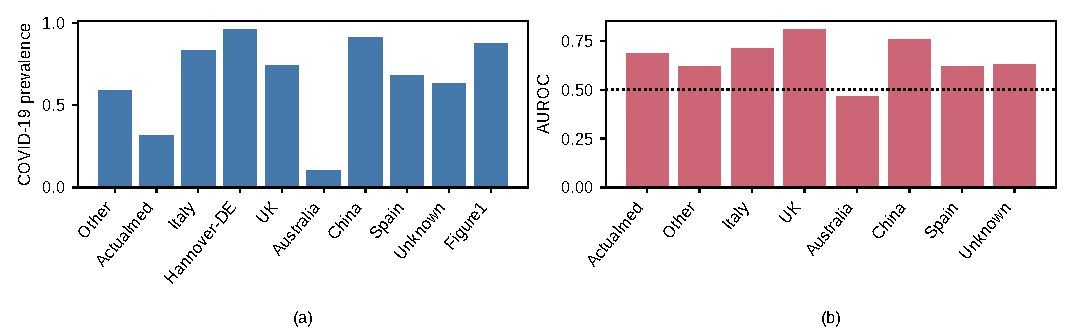
\includegraphics[width=\textwidth]{fig_diagnostics.pdf}
\caption{(a) COVID-19 prevalence per data source. (b) AUROC for predicting the diagnosis on a held-out site from five acquisition statistics alone; the dotted line marks chance (0.5).}\label{fig:diag}
\end{figure*}

\subsection{No Method Significantly Beats ERM}\label{sec:noerm}
\erm{} reached an AUROC of $\TErmAurocDev$ on the development folds and $\TErmAurocConf$ on the confirmation folds (Table~\ref{tab:main}, Fig.~\ref{fig:methods}). Paired differences to \erm{} are small, and every interval includes zero. GroupDRO is nominally best at $+\TGroupdroDiffVsErm$ [$\TGroupdroLo$, $\TGroupdroHi$], followed by SIDL-phys at $+\TSidlPhysDiffVsErm$ [$\TSidlPhysLo$, $\TSidlPhysHi$]. The other six methods sit at or below \erm{}, and SIDL-full, the variant that combines all components, is the lowest at $\TSidlFullDiffVsErm$ [$\TSidlFullLo$, $\TSidlFullHi$]. The upper bounds rule out gains above about $0.055$ for every method. Per-site values are listed in Appendix~\ref{app:perfold}.

Rankings are unstable: method means correlate only $\rankCorrDevConf$ (Spearman) between the development and confirmation folds. Site-profile augmentation tied \erm{} on development folds ($\TSiteProfileAugAurocDev$ vs.\ $\TErmAurocDev$) and fell below it on confirmation folds ($\TSiteProfileAugAurocConf$ vs.\ $\TErmAurocConf$), whereas SIDL-phys moved the other way. GroupDRO also has a higher balanced accuracy ($\TGroupdroBalAcc$ vs.\ $\TErmBalAcc$) and a better worst-site AUROC ($\TGroupdroWorstFold$ vs.\ $\TErmWorstFold$). We treat both as exploratory, because \erm{}'s worst site has only 6 positives, PAI does not share the gain, and balanced accuracy depends on an operating point that group reweighting shifts. In pilot runs, whole-batch full-strength augmentation cost up to $0.083$ AUROC on the development folds ($0.675$ vs.\ $0.758$). Making the augmentation per-sample and mild removed the drop but never produced a gain. Stronger invariance also hurt: PAI with adversary weight $0.5$ instead of the frozen $0.1$ lost $0.036$--$0.051$ AUROC on the development folds.
\begin{table*}[!tb]\centering\footnotesize
\caption{Leave-One-Site-Out Task Metrics for the CNN}\label{tab:main}
\tabin{main.tex}
\tabnote{Mean over held-out sites of the two-seed mean. $\Delta$ is the paired AUROC difference to ERM over eight sites with a hierarchical bootstrap 95\% interval. Worst fold is the lowest per-site AUROC. Balanced accuracy and the expected calibration error (ECE) use the argmax decision.}
\end{table*}
\begin{figure*}[!tb]\centering
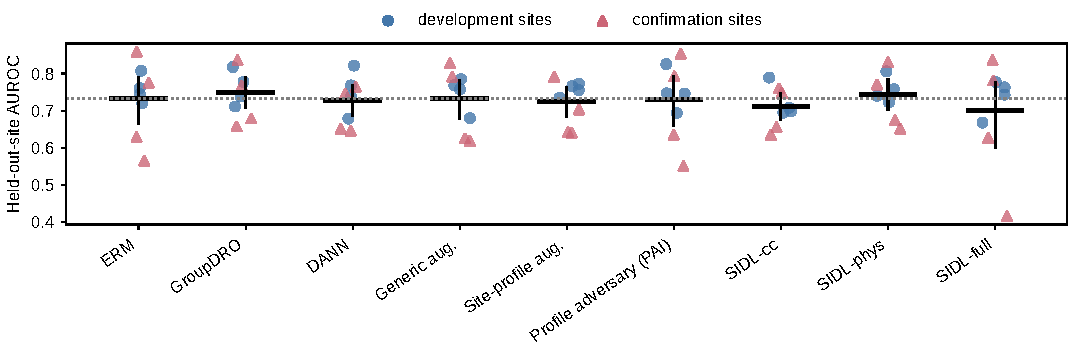
\includegraphics[width=\textwidth]{fig_methods.pdf}
\caption{Held-out AUROC per CNN method. Markers show sites (circles: development; triangles: confirmation); the horizontal bar and vertical line show the mean and the bootstrap interval over sites, and the dotted line marks the ERM mean.}\label{fig:methods}
\end{figure*}

\subsection{Controlled Label Shift}\label{sec:synthls}
On the semisynthetic benchmark, where image content is identical and the transforms are known, adversarial alignment hurts most at the largest prior spread ($0.4$). Against \erm{}, DANN loses $\synthDiffDann$ [$\synthDiffDannLo$, $\synthDiffDannHi$] and cDANN loses $\synthDiffCdann$ [$\synthDiffCdannLo$, $\synthDiffCdannHi$], whereas cDANN with prior reweighting ends at $\synthDiffCdannP$ [$\synthDiffCdannPLo$, $\synthDiffCdannPHi$], which cannot be told apart from \erm{}. Reweighting alone gains $+\synthDiffErmP$ [$\synthDiffErmPLo$, $\synthDiffErmPHi$]. That interval excludes zero, but it rests on six units and four uncorrected comparisons, and the same reweighting did not help the pretrained heads on real sites (Section~\ref{sec:frozen}). The ordering matches theory, with unconditional alignment hurting most and class-conditional alignment with reweighting hurting least (Table~\ref{tab:synthls}).

A weaker adversary costs less. At weight $0.5$, the adversaries lose $\synthNoShiftLossMin$--$\synthNoShiftLossMax$ AUROC even with no label shift, but at weights of $0.1$ and $0.02$ both DANN and cDANN with reweighting stay within $0.02$ of \erm{} at spread $0.4$ (Table~\ref{tab:synthadv}). Neither beats \erm{} with reweighting alone ($0.770$ against at most $0.756$), so in this experiment the gain comes from the reweighting and not from the adversary. With six units per cell, we cannot claim that the class-conditional adversary helps.
\begin{table}[!t]\centering\footnotesize
\caption{Semisynthetic Label-Shift Sweep}\label{tab:synthls}
\tabin{synth_labelshift.tex}
\tabnote{Held-out AUROC on virtual sites V0, V2, and V4 (two seeds, adversary weight $0.5$).}
\end{table}
\begin{table}[!t]\centering\footnotesize\setlength{\tabcolsep}{2pt}
\caption{Adversary Weight in the Semisynthetic Sweep}\label{tab:synthadv}
\tabin{synth_advweight.tex}
\tabnote{Held-out AUROC at prior spreads of $0$ and $0.4$ (six units per cell). $\lambda$ is the weight of the gradient-reversal layer; \erm{} has no adversary.}
\end{table}

\subsection{A Frozen Pretrained Encoder Gives the Same Answer}\label{sec:frozen}
Replacing the CNN with a frozen chest-radiograph encoder did not change the conclusion. Over eight sites, the pretrained head is not clearly better than the CNN (AUROC $\RtPreAll$ vs.\ $\RtCnnAll$; difference $\RtPreVsCnnAll$ [$\RtPreVsCnnAllLo$, $\RtPreVsCnnAllHi$]). It is better at five sites, most clearly Australia and China, and worse at Actualmed, Italy, and UK (Fig.~\ref{fig:round2}a). Its standing against the CNN also differs between fold sets ($\RtPreDev$ vs.\ $\RtCnnDev$ on development, $\RtPreConf$ vs.\ $\RtCnnConf$ on confirmation).

None of the invariance heads beat \erm{} on the embedding (Table~\ref{tab:heads}). GroupDRO again had the largest gain, $\RtGdroDiff$ [$\RtGdroLo$, $\RtGdroHi$] ($\RtGdroDev$ on development folds and $\RtGdroConf$ on confirmation folds). Its interval touches zero, and it is the best of eight uncorrected comparisons. The class-conditional adversary, CORAL, DANN, and prior reweighting stayed within $0.006$ of \erm{}. Adversary plus prior reweighting was lower ($\RtCdannPDiff$), and site centering, which needs unlabeled target images, was clearly worse ($\RtCenterDiff$ [$\RtCenterLo$, $\RtCenterHi$]). Every upper bound was below $0.04$. The embedding still carries site information: a patient-grouped linear classifier names the source among ten with an accuracy of $\RdSiteAcc$ ($\RdSiteMaj$ for the majority source).
\begin{table}[!t]\centering\footnotesize\setlength{\tabcolsep}{1.5pt}
\caption{Training Methods on the Frozen Pretrained Embedding}\label{tab:heads}
\tabin{r2_heads.tex}
\tabnote{Five seeds; settings fixed before the confirmation run. $\Delta$ is the paired AUROC difference to the pretrained ERM head over eight sites with a hierarchical bootstrap 95\% interval.}
\end{table}

\subsection{Combining the Two Encoder Families}\label{sec:combine}
The two model families fail at different sites. The CNN is weakest on Australia and Other, and the pretrained head on Actualmed and UK. Averaging five CNNs with five pretrained heads gave the best mean and the best worst-site AUROC (Table~\ref{tab:models}, Fig.~\ref{fig:round2}a). Both pre-specified comparisons pointed the same way on both fold sets, and neither was significant. Against the five-CNN ensemble the difference is $\RtEnsVsCnnEnsAll$ [$\RtEnsVsCnnEnsAllLo$, $\RtEnsVsCnnEnsAllHi$] (development $\RtEnsVsCnnEnsDev$, confirmation $\RtEnsVsCnnEnsConf$), and against a single CNN it is $\RtEnsVsCnnAll$ [$\RtEnsVsCnnAllLo$, $\RtEnsVsCnnAllHi$] (development $\RtEnsVsCnnDev$, confirmation $\RtEnsVsCnnConf$).

Three cautions apply. On the confirmation folds, the pretrained five-head ensemble was as good as the combination ($\RtPreEnsConf$ vs.\ $\RtEnsConf$), so the data cannot separate ``combining helps'' from ``pretraining helps''. Seed averaging alone also helps: the five-CNN ensemble beats the single CNN by $\RtCnnEnsVsCnnAll$ [$\RtCnnEnsVsCnnAllLo$, $\RtCnnEnsVsCnnAllHi$]. Finally, the lead over a single CNN depends heavily on the two smallest test sets (Section~\ref{sec:robust}). We treat the combination as a suggestive direction and not as a result.
\begin{table*}[!tb]\centering\footnotesize
\caption{Encoder Families and Their Ensembles}\label{tab:models}
\tabin{r2_models.tex}
\tabnote{Held-out AUROC averaged over the four development sites, the four confirmation sites, and all eight (five seeds). $\Delta$ is the paired difference to the single CNN with a hierarchical bootstrap 95\% interval (2000 replicates).}
\end{table*}
\begin{figure*}[!tb]\centering
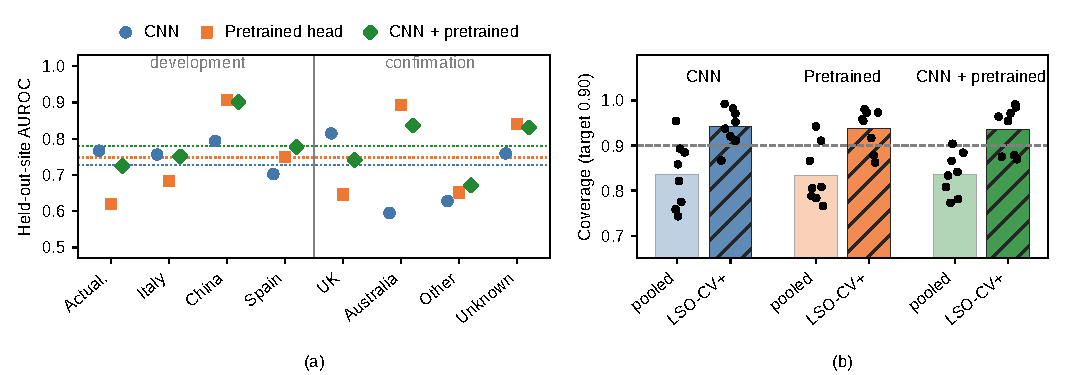
\includegraphics[width=\textwidth]{fig_round2.pdf}
\caption{(a) Held-out AUROC for the single CNN, the single pretrained head, and their combination at each site; dotted lines are means over eight sites. (b) Conformal coverage on each held-out site at $\alpha=0.1$ for seen-site pooled and LSO-CV+ calibration (bars: mean of eight sites; dots: sites; dashed: target).}\label{fig:round2}
\end{figure*}

\subsection{Conformal Sets Under-Cover Unseen Sites}\label{sec:conf}
Sets calibrated on seen-site validation data miss the target (Table~\ref{tab:conf}, Fig.~\ref{fig:conf}). Mean coverage at the $0.90$ target is $\CPooledCovMean$ for pooled and $\CSiteBalancedCovMean$ for site-balanced calibration. The worst site gets about $\CPooledCovMin$, and $\CPooledNUnder$ of $\CPooledN$ sites are more than five points short. The pattern appears in both fold sets (pooled coverage is $0.829$ on development and $0.843$ on confirmation folds).

Worst-site calibration restores the mean ($\CWorstSiteCovMean$) but leaves two sites short, with the lowest coverage ($\CWorstSiteCovMin$) at ``Other''. LSO-CV+ reaches a mean coverage of $\CLsoCvplusCovMean$, and its lowest site coverage is $\CLsoCvplusCovMin$, with no site more than five points short. Its mean set size is $\CLsoCvplusSize$, against $\CPooledSize$ for pooled calibration. It over-covers at seven of the eight sites. LSO-split lands nearer the target on average ($\CLsoSplitCovMean$) but leaves one site at $\CLsoSplitCovMin$.

These calibrations differ in operating point and not in efficiency. Interpolated at $90\%$ coverage, set size lies between $\CLsoSplitSizeAtCov$ and $\CSiteBalancedSizeAtCov$ for \emph{every} calibration (pooled $\CPooledSizeAtCov$, LSO-CV+ $\CLsoCvplusSizeAtCov$). The development folds had suggested that LSO-CV+ was about $4\%$ smaller at matched coverage, and the confirmation folds did not repeat that. Its benefit is therefore safety. Whether sets about $26\%$ larger are worth a six-point average shortfall (up to sixteen points at the worst site) depends on the application. Two other ideas failed on development folds and were dropped. One weighted the calibration scores by a density ratio of the acquisition profile (coverage $0.834$ vs.\ $0.829$ for pooled). The other corrected for estimated label shift~\cite{saerens2002adjusting,podkopaev2021distribution} (coverage $0.813$ with an expectation--maximization prior and $0.845$ with the oracle prior, with worse balanced accuracy).
\begin{table*}[!tb]\centering\footnotesize
\caption{Conformal Prediction for the CNN ERM Model}\label{tab:conf}
\tabin{conformal.tex}
\tabnote{Eight held-out sites, $\alpha=0.1$ (target $0.90$), two seeds. Sites $<$0.85 counts sites with more than five points under target; the last three columns use the $\alpha$ grid. Rows 1--3 were calibrated on the seen-site validation data, and rows 4--8 used leave-site-out scores.}
\end{table*}
\begin{figure*}[!tb]\centering
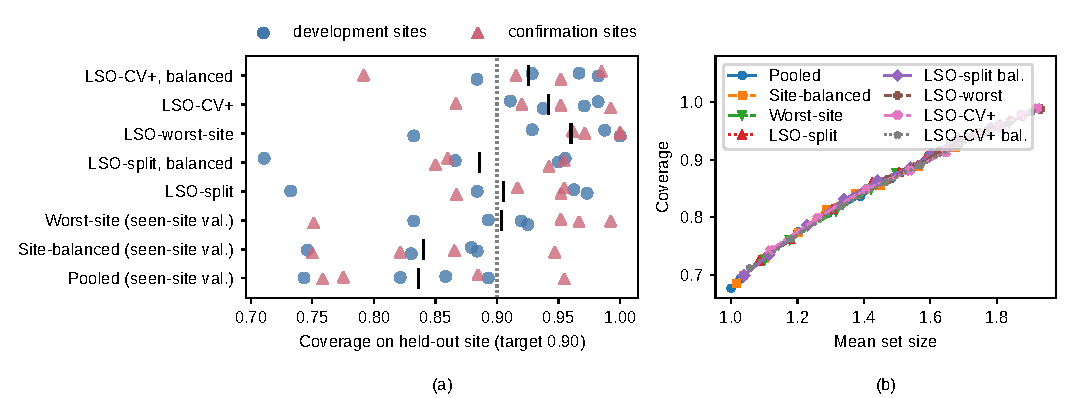
\includegraphics[width=\textwidth]{fig_conformal.pdf}
\caption{(a) Coverage of each held-out site at $\alpha=0.1$ (vertical bar: mean; dotted line: $0.90$ target). (b) Coverage versus mean set size over the $\alpha$ grid; all calibrations lie on nearly one curve.}\label{fig:conf}
\end{figure*}

\emph{The same holds for the pretrained head and the ensemble} (Table~\ref{tab:confall}, Fig.~\ref{fig:round2}b). Pooled coverage is $\RcPrePooledCov$ for the pretrained head and $\RcEnsPooledCov$ for the ensemble, with $\RcPrePooledUnder$ of 8 sites more than five points short in both. LSO-CV+ reaches $\RcPreCvplusCov$ and $\RcEnsCvplusCov$ with no such site. A better ranking model therefore does not close the coverage gap. At matched $90\%$ coverage, the ensemble's sets are somewhat smaller ($\RcEnsPooledSninety$--$\RcEnsCvplusSninety$ against $\RcCnnPooledSninety$--$\RcCnnCvplusSninety$ for the CNN). The paired per-site difference for LSO-CV+ is $\RcEnsCnnCvplusDiff$ [$\RcEnsCnnCvplusLo$, $\RcEnsCnnCvplusHi$], with smaller sets at $\RcEnsCnnCvplusN$ of 8 sites, so we again call it a direction.

\begin{table*}[!tb]\centering\footnotesize
\caption{Conformal Calibration Across Model Families}\label{tab:confall}
\tabin{r2_conformal.tex}
\tabnote{Eight sites, two seeds, $\alpha=0.1$. Cov.\ is mean coverage with, in parentheses, the number of sites more than five points under the $0.90$ target; Size is mean set size; @90\% is set size interpolated at $90\%$ coverage over the $\alpha$ grid.}
\end{table*}

\subsection{Why: Validation Optimism}\label{sec:why}
For the CNN \erm{} model, we compared three AUROC values: the one on seen-site validation data, the leave-site-out estimate (inner models scored on the sites they did not see), and the actual held-out AUROC (Fig.~\ref{fig:optim}). Over $\ONUnits$ site-seed units, seen-site validation overstates held-out AUROC by $\OMeanSignedSeen$ on average (absolute error $\OMaeSeen$). The leave-site-out estimate is nearly unbiased ($\OMeanSignedLso$; absolute error $\OMaeLso$). The pretrained head shows the same optimism ($\RdValAuc$ on seen-site validation vs.\ $\RdTestAuc$ on held-out sites, a gap of $\RdOptim$ over 40 units).

Neither estimate ranks the sites (Spearman correlation with actual AUROC for the CNN: $\ORhoSeen$ and $\ORhoLso$). Actual AUROC ranges from $0.56$ to $0.86$, whereas the leave-site-out estimate stays between $0.72$ and $0.75$, so it describes a typical unseen site and not a particular one. The per-site optimism gap and pooled-conformal coverage are rank-correlated in the expected direction ($\ORhoGapCov$ over eight sites). That is consistent with optimism driving under-coverage, but it is not significant at this sample size. Averaging the inner models, a free by-product, gives an AUROC of $\ensAurocEns$ vs.\ $\ensAurocFull$ for the single model ($\ensDAuroc$ [$\ensDAurocLo$, $\ensDAurocHi$]), which is no significant gain.
\begin{figure}[!t]\centering
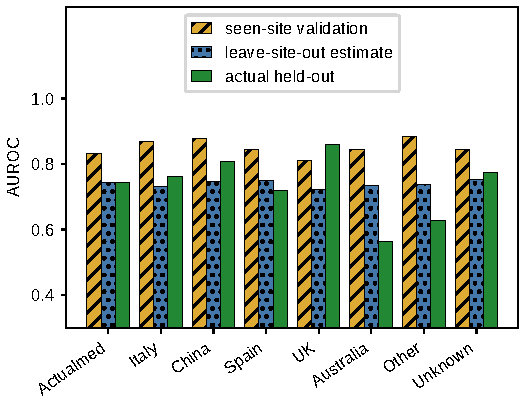
\includegraphics[width=\columnwidth]{fig_optimism.pdf}
\caption{AUROC of the CNN \erm{} model estimated on the seen-site validation data, by leave-site-out models, and obtained on the held-out site (two-seed mean).}\label{fig:optim}
\end{figure}

\subsection{Simulated Shifts Are Poor Stand-Ins}\label{sec:simshift}
On the semisynthetic benchmark with three acquisition-severity levels, seen-site pooled calibration covers $\synthPooledCovMin$--$\synthPooledCovMax$ at the $0.90$ target (Table~\ref{tab:synthconf}), unlike the $\CPooledCovMean$ on real sites, and its lowest single site is $0.875$. The leave-site-out rules over-cover instead (LSO-CV+ reaches $\synthCvplusCovMin$--$\synthCvplusCovMax$ with sets $9$--$17\%$ larger than pooled), and only worst-site calibration at the highest severity falls a little short ($0.881$). The real under-coverage therefore probably comes from differences between sites that our simulation lacks, such as patient mix, case selection, labeling, and image provenance. A calibration method that was checked only on simulated acquisition shifts would have looked fine.
\begin{table}[!t]\centering\footnotesize\setlength{\tabcolsep}{1.5pt}
\caption{Conformal Coverage on the Semisynthetic Benchmark}\label{tab:synthconf}
\tabin{synth_conformal_short.tex}
\tabnote{Mean coverage over six units at $\alpha=0.1$ (target $0.90$), with the lowest single-site coverage in parentheses, for three acquisition severities at prior spread $0.25$. Size is the mean set size for pooled and LSO-CV+ calibration.}
\end{table}

\subsection{Robustness Checks}\label{sec:robust}
We added five checks that a careful reviewer would ask for. None changed a setting or any result reported above.

\emph{How uncertain is the coverage?} Table~\ref{tab:covci} gives hierarchical-bootstrap intervals for the mean coverage at $\alpha=0.1$. With pooled calibration, the interval excludes the $0.90$ target for all three model families, and at most $\RvMaxPAbove$ of the bootstrap replicates reach $0.90$. The LSO-CV+ intervals sit at or above the target (the ensemble's lower end is $\RvEnsCvplusLo$). Worst-site and LSO-split calibration cannot be told apart from the target: for the CNN, worst-site coverage is $\CWorstSiteCovMean$ with an interval of $[\RvCnnWorstLo, \RvCnnWorstHi]$.

\emph{Which class is missed?} The shortfall is not spread evenly. With pooled calibration, non-COVID images are covered $\RvCnnPooledOther$--$\RvEnsPooledOther$ of the time, but COVID images $\RvCnnPooledCovid$--$\RvEnsPooledCovid$ (Table~\ref{tab:covci}). LSO-CV+ brings non-COVID coverage to $\RvEnsCvplusOther$--$\RvCnnCvplusOther$ and over-covers COVID images ($\RvCnnCvplusCovid$--$\RvEnsCvplusCovid$). A marginal guarantee can therefore hide a large gap in one class.
\begin{table}[!t]\centering\footnotesize\setlength{\tabcolsep}{1.5pt}
\caption{Conformal Coverage With Bootstrap Intervals}\label{tab:covci}
\tabin{r2_coverage_ci.tex}
\tabnote{Mean over eight held-out sites at $\alpha=0.1$ with a hierarchical bootstrap 95\% interval (3000 replicates, seeds averaged), and mean coverage within each class (over sites with at least five images of the class). Pooled calibration uses the seen-site validation data.}
\end{table}

\emph{What if the two tiny sites are removed?} China has 5 negative images and Australia has 6 positive ones. On the remaining six sites, no CNN method is above \erm{} (the largest loss is $\RvSixCnnWorstDiffMin$), and the GroupDRO gain falls from $+\TGroupdroDiffVsErm$ to $\RvSixGdroCnn$ [$\RvSixGdroCnnLo$, $\RvSixGdroCnnHi$]. On the pretrained embedding, GroupDRO rises to $\RvSixGdroPre$ [$\RvSixGdroPreLo$, $\RvSixGdroPreHi$], the only six-site interval that excludes zero. We picked that subset after seeing the results, so we do not treat it as confirmatory. The ensemble's lead over a single CNN shrinks from $\RtEnsVsCnnAll$ to $\RvSixEnsCnn$ [$\RvSixEnsCnnLo$, $\RvSixEnsCnnHi$], because its per-site gains are largest at Australia and China (Fig.~\ref{fig:round2}a). Its worst-site advantage persists in a smaller form ($\RvSixWorstEns$, against $\RvSixWorstCnn$ for the CNN and $\RvSixWorstPre$ for the pretrained head). The coverage findings do not depend on these two sites. On the six sites, pooled coverage is $\RvSixCnnPooled$, $\RvSixPrePooled$, and $\RvSixEnsPooled$ for the CNN, pretrained head, and ensemble, against $\RvSixCnnCvplus$, $\RvSixPreCvplus$, and $\RvSixEnsCvplus$ for LSO-CV+.

\emph{Does anything survive multiple testing?} The second study made $\RvNComparisons$ comparisons: eight heads against \erm{}, the ensemble against the CNN, the ensemble against the five-CNN ensemble, and the pretrained head against the CNN. The smallest two-sided bootstrap $p$-value is $0.028$, for site centering, which is worse than \erm{}. GroupDRO follows at $\RvRawGdro$. After Holm correction, the smallest adjusted $p$-value is $\RvHolmMin$ (GroupDRO: $\RvHolmGdro$), so no difference is significant. The eight CNN comparisons already have intervals that include zero without any correction.

\emph{Does the uncorrected sharpness statistic matter?} The sharpness statistic in the site profile is not corrected for noise, so added noise raises it (Section~\ref{sec:synth}). We repeated site-profile augmentation and PAI on all eight sites with a noise-corrected statistic and left every other setting frozen. Site-profile augmentation moved from $\cmpPhysOldDiff$ to $+\cmpPhysDiff$ against \erm{} [$\cmpPhysLo$, $\cmpPhysHi$], and PAI went from $\cmpPaiOldDiff$ to $\cmpPaiDiff$ [$\cmpPaiLo$, $\cmpPaiHi$]. Both intervals include zero. Most of the change for site-profile augmentation comes from the UK site, where one of the two reported seeds had an AUROC of only $\cmpUkLowSeed$, so we read it as seed variance and not as evidence that the correction helps. The label-leak AUROC was $\cmpLeakOld$ with the original statistic and $\cmpLeakNew$ with the corrected one. This check was post hoc and was not used for any decision.

\section{Discussion}\label{sec:discussion}
\subsection{Answers to the Research Questions}
Table~\ref{tab:rq} maps each question to its evidence, and the paragraphs below give the answers in more detail.
\begin{table}[!t]\centering\footnotesize
\caption{Research Questions, Evidence, and Answers}\label{tab:rq}
\begin{tabular}{@{}p{0.06\columnwidth}p{0.4\columnwidth}p{0.48\columnwidth}@{}}
\toprule
 & Evidence & Answer \\
\midrule
RQ1 & Secs.~\ref{sec:noerm}, \ref{sec:synthls}; Tables~\ref{tab:main}, \ref{tab:synthls}; Fig.~\ref{fig:methods} & No gain over \erm{}; every interval includes zero \\
RQ2 & Secs.~\ref{sec:frozen}, \ref{sec:combine}; Tables~\ref{tab:heads}, \ref{tab:models} & Same answer; the ensemble's lead is not significant \\
RQ3 & Secs.~\ref{sec:conf}, \ref{sec:simshift}, \ref{sec:robust}; Tables~\ref{tab:conf}--\ref{tab:covci} & Seen-site calibration under-covers; site-fold CV+ avoids the worst cases \\
RQ4 & Sec.~\ref{sec:why}; Fig.~\ref{fig:optim} & Seen-site validation is optimistic \\
\bottomrule
\end{tabular}
\end{table}
\emph{RQ1: do invariance methods help at unseen hospitals?} Not on this benchmark. None of eight methods beat \erm{} by more than noise, and the upper bounds of the intervals rule out gains above about $0.055$ AUROC (Section~\ref{sec:noerm}). GroupDRO had the largest nominal gain, but it vanishes when the two smallest test sites are removed (Section~\ref{sec:robust}). Acquisition statistics do leak the label, and model scores follow them within class (Section~\ref{sec:leak}). Still, the methods that lower this reliance did not improve accuracy, so we cannot say that the shortcut explains the accuracy loss. Controlled label shift gave a similar picture. At the default weight every adversary was below \erm{}, the class-conditional version with reweighting lost least, and at weaker weights no adversary beat \erm{} with reweighting alone (Section~\ref{sec:synthls}).

\emph{RQ2: does a frozen pretrained encoder change this?} No. None of the eight heads beat \erm{} on the embedding, and gains above about $0.04$ are unlikely (Section~\ref{sec:frozen}). GroupDRO again had the largest nominal gain, but it does not survive correction for multiple comparisons. Averaging the CNN with the pretrained head gave the best mean AUROC, but the lead is not significant and rests largely on two tiny test sites (Sections~\ref{sec:combine} and~\ref{sec:robust}).

\emph{RQ3: do conformal sets keep their coverage at an unseen site?} Not with seen-site calibration. Mean coverage was about six points below the $0.90$ target for the CNN, the pretrained head, and their ensemble, and the bootstrap intervals exclude the target (Sections~\ref{sec:conf} and~\ref{sec:robust}). The shortfall sits mostly in the non-COVID class. Calibrating with sites as folds (LSO-CV+) removed the worst shortfalls at the price of larger sets, and a simulated acquisition shift did not reproduce the effect (Section~\ref{sec:simshift}).

\emph{RQ4: why do seen-site estimates mislead?} A model has already fitted the sites on which it is validated. Seen-site validation overstated held-out AUROC by $\OMeanSignedSeen$ for the CNN and by $\RdOptim$ for the pretrained head, whereas the leave-site-out estimate was nearly unbiased on average (Section~\ref{sec:why}). The same optimism is a likely reason for the under-coverage, although the rank correlation across eight sites supports this only weakly. Neither estimate tells us which site will be hard.

\subsection{Why Invariance May Not Have Helped}
We suspect that invariance fails here because the data are tiny (held-out sites of 52--207 images), the label-correlated signal sits mostly within sites, and adversaries add optimization noise that small heads cannot afford. A further possibility is that sites differ in how cases were selected and labeled, which no image-level invariance can remove. A study of chest-radiograph datasets found label differences to matter more than image differences~\cite{cohen2020limits}, and a study of pathology images traced lost exchangeability to disagreement between annotators~\cite{boman2026conformal}. We did not test any of these explanations.

\subsection{Practical Guidance}
Three suggestions follow for anyone building a multi-site model. First, report leave-one-site-out results with intervals that respect small sites, and keep the sites used for the final report out of tuning. Seen-site validation overstated AUROC by $\OMeanSignedSeen$ here. Second, treat nominal coverage from seen-site calibration as optimistic for unseen sites. On this benchmark it fell about six points short on average, and the shortfall was concentrated in the non-COVID class, so check coverage by class if a missed class is costly. Third, if under-coverage is costly, calibrate with sites as folds (LSO-CV+) and accept sets about $26\%$ larger. That rule made the sets safer, not more efficient. Before investing in an invariance method, compare it with \erm{} and with a cheap ensemble under the same frozen protocol. On these data, neither adversaries nor augmentation moved the result.

\subsection{Threats to Validity}
\emph{Internal validity.} Eight sites and tiny test sets give wide intervals, so ``no significant difference'' does not show equivalence below roughly $0.03$ AUROC. The intervals in the tables are not corrected for multiplicity (Section~\ref{sec:robust} reports Holm-adjusted $p$-values). The development/confirmation split was ours and not random, tuning budgets were modest, and a better-tuned variant could still help. The CNN confirmation results were known before the pretrained family was designed. The profile estimators are proxies for scanner physics, and the semisynthetic cells have only six units each. One conclusion from them, that prior reweighting was neutral, changed when image reuse was removed (Section~\ref{sec:synth}), which shows how fragile such single cells are.

\emph{External validity.} The study covers one modality and one binary task, and the data are public, retrospective, and assembled from publications and case reports. Absolute AUROC is therefore not clinically meaningful, and ``Other'' and ``Unknown'' mix institutions. The collection is a merged public one of the kind that a systematic review warns against~\cite{roberts2021common}, which is why we use it only to test site shortcuts. The CNN saw images reduced to $64\times64$ pixels, which may remove the fine texture and noise cues that site-profile augmentation targets, although the pretrained family used $224\times224$ images and gave the same answer. Our environment could not reach larger or credentialed datasets and had no graphics processor, and we used no private data. The pretrained encoder was frozen and not fine-tuned, and we did not check whether images in this benchmark also appear in its pretraining collections.

\emph{Construct validity.} A site is a metadata label (institution or country) and not a measured scanner. No leave-site-out conformal rule has a finite-sample guarantee under site shift. We measured coverage marginally and by class, not conditionally on patient or site-level covariates. Larger data, more sites, and fine-tuned encoders would be needed to show whether invariance helps.

\section{Conclusion}
On this benchmark, making a model invariant to scanner and institution did not help at unseen hospitals, for a small convolutional network and for a frozen pretrained encoder alike. What carries over to other studies concerns evaluation and uncertainty. Validation on seen sites and standard conformal calibration both flatter the result at a new site, and a rule that treats sites as the unit of resampling is a practical safeguard at the price of larger prediction sets. Three questions remain open: whether invariance helps with more and larger sites and with fine-tuned encoders, whether a theory of exchangeability across sites can give finite-sample guarantees, and whether averaging models of different origin keeps its advantage once the tiny test sets are replaced. Answering them needs multi-site data with patient-level and scanner-level metadata, which this benchmark lacks.

\appendix[Per-Site AUROC of the CNN Methods]\label{app:perfold}
Table~\ref{tab:perfold} lists the held-out AUROC of every CNN method at each of the eight sites; Fig.~\ref{fig:methods} plots the same values.

\begin{table*}[!tb]\centering\footnotesize
\caption{Held-Out AUROC per Site}\label{tab:perfold}
\tabin{perfold.tex}
\tabnote{Two-seed mean. Superscripts: d = development fold, c = confirmation fold.}
\end{table*}

\section*{Acknowledgment}
The artificial intelligence (AI) system Claude (Anthropic), used through the Claude Code environment, wrote the experiment code, ran the experiments, produced the tables and figures, and drafted all sections of this manuscript, including the Related Work and Discussion. It also revised the prose after an internal review and ran the robustness checks. The authors directed the work, edited the text for clarity and wording, and are responsible for the content. All reported numbers were generated by the released code. The open-source LanguageTool grammar checker was used on the compiled text. The chest-radiograph encoder used in the second experiment family is a model component and is cited as such.

\bibliographystyle{IEEEtran}
\bibliography{refs}

\end{document}
